\section{Development Environment}

Figure \ref{fig:devenvironment} outlines all components of the development environment. The Service Cutter is developed with Java 8 using Eclipse Mars~\cite{eclipsemars}. \gls{HSR} has provided a \gls{VM} on which the \gls{docker} images are running. On the same server a \gls{CI} Jenkins server pulls for changes from the Git repositories on GitHub to build and test the different projects. The Docker images are built using a Maven plugin on Jenkins and then pushed into the local Docker repository. Table \ref{tab:vm} indicates the software installed by us on the server.


\begin{table}[H]
\begin{center}
\begin{tabular}
{|p{100pt} p{80pt}|}
\hline \textbf{Software} & \textbf{Version} \\ 
\hline Java & 1.8.0\_60 \\ 
\hline Jenkins & 1.629 \\ 
\hline Docker & 1.8.2 \\ 
\hline Docker Compose & 1.4.1 \\
\hline Apache Maven & 3.0.5 \\
\hline Node.js & 0.10.25 \\
\hline NPM & 1.3.10 \\
\hline 
\end{tabular} 
\caption{Installed software on sinv-56064.edu.hsr.ch (152.96.56.64)}
\label{tab:vm}
\end{center}
\end{table}

\begin{figure}[H]
	\centering{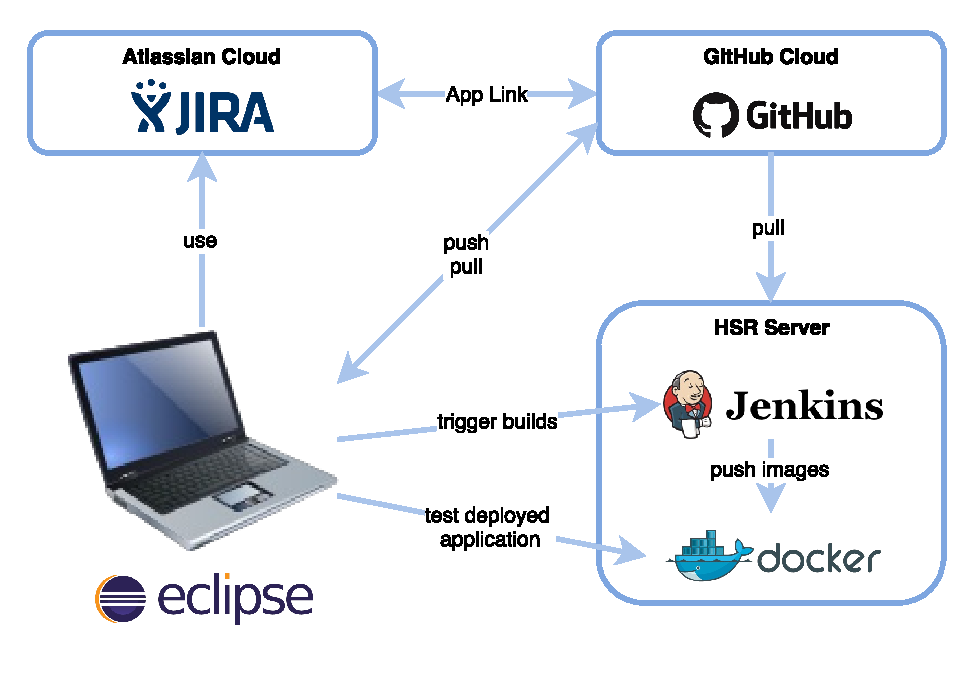
\includegraphics[scale=0.7]{diagrams/DevelopmentEnvironment.pdf}}
	\caption{Development Environment}
	\label{fig:devenvironment}
\end{figure}
